\section{Appendix}

Code from Kalman Filter. In higher dimensions mutliplication would need to be matrix dot product. Constants set as parametres for easier testing.
\begin{verbatim}
def kf_predict(X, S, U):
	x = A*X + B*U
	s = A*S*A + R
	return x, s

def kf_update(X, S, Z):
	k = S*C/(C*S*C+Q)
	x = X+k*(Z-C*X)
	s = (1-C*k)*S
	return x, s
\end{verbatim}


\begin{figure}[tbd]
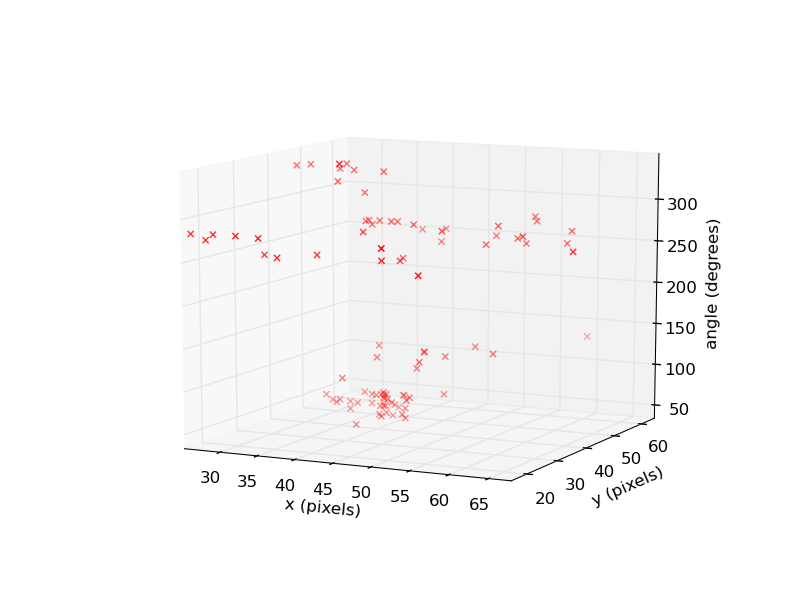
\includegraphics[width=0.6\textwidth]{images/training_data.png}
\caption{\label{occupied} Sample of Training Data}
\end{figure}


\begin{figure}[tbd]
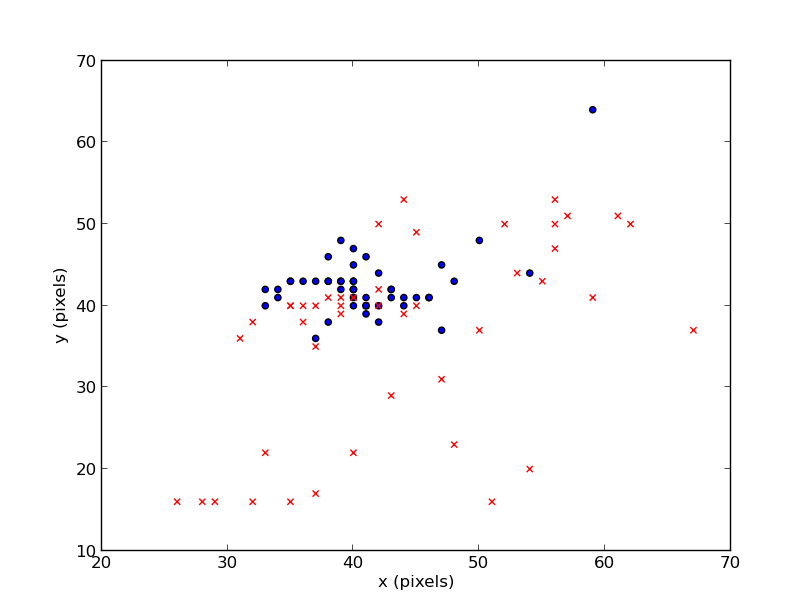
\includegraphics[width=0.5\textwidth]{images/xy_training_coloured.png}
\caption{\label{occupied} Labelled Training Data}
\end{figure}